\chapter{GIỚI THIỆU BÀI TOÁN PHÁT HIỆN, PHÂN LOẠI VÀ THEO DÕI PHƯƠNG TIỆN GIAO THÔNG}
\label{chap:gioithieu}

\section{Giới thiệu bài toán}

Bài toán của đề tài nhận đầu vào là video từ một camera giao thông đặt cố định, nhìn chéo xuống mặt đường từ trên cao,
độ phân giải 1920×1080. Với mỗi frame, hệ thống cần trả lời ba câu hỏi: trong ảnh có những phương tiện nào và nằm ở
đâu, mỗi phương tiện thuộc loại gì, và phương tiện nào ở frame này là cùng một xe với phương tiện nào ở frame trước.
Tương ứng với ba câu hỏi đó là ba bài toán con.

\textbf{Phát hiện đối tượng (object detection).} Mô hình nhận một ảnh và trả về danh sách hình chữ nhật bao quanh
(bounding box, gọi tắt là box) của từng phương tiện, mỗi box kèm một điểm tin cậy trong khoảng $[0, 1]$.

\textbf{Phân loại.} Mỗi box được gán một trong bốn lớp: xe máy (\texttt{motorbike}), ô tô (\texttt{car}), xe buýt
(\texttt{bus}) và xe tải (\texttt{truck}). Trong các mô hình phát hiện hiện đại, phân loại được làm cùng lúc với
phát hiện: đầu ra của mạng cho cả toạ độ box lẫn xác suất từng lớp. Box xe máy được quy ước bao cả người lái, vì từ
góc camera giao thông người và xe máy là một khối khó tách.

\textbf{Theo dõi đa đối tượng (multi-object tracking, MOT).} Thuật toán theo dõi nối các box của cùng một xe qua các
frame liên tiếp và gán cho mỗi xe một mã định danh (ID) không đổi trong suốt thời gian xe xuất hiện. Đề tài theo
hướng \emph{tracking-by-detection}: chạy mô hình phát hiện trên từng frame, rồi ghép box của frame mới với các quỹ đạo
đang theo dõi dựa trên vị trí dự đoán.

Khi đã có ID ổn định cho từng xe, hệ thống đếm được số xe đi qua một vạch ảo theo từng lớp và từng hướng. Đếm xe là
ứng dụng minh hoạ của kết quả theo dõi; trọng tâm đánh giá của đề tài vẫn là độ chính xác phát hiện (mAP) và chất
lượng theo dõi (HOTA, MOTA, IDF1). Hình~\ref{fig:demo-pvd} là một frame đầu ra của hệ thống.

\begin{figure}[H]
  \centering
  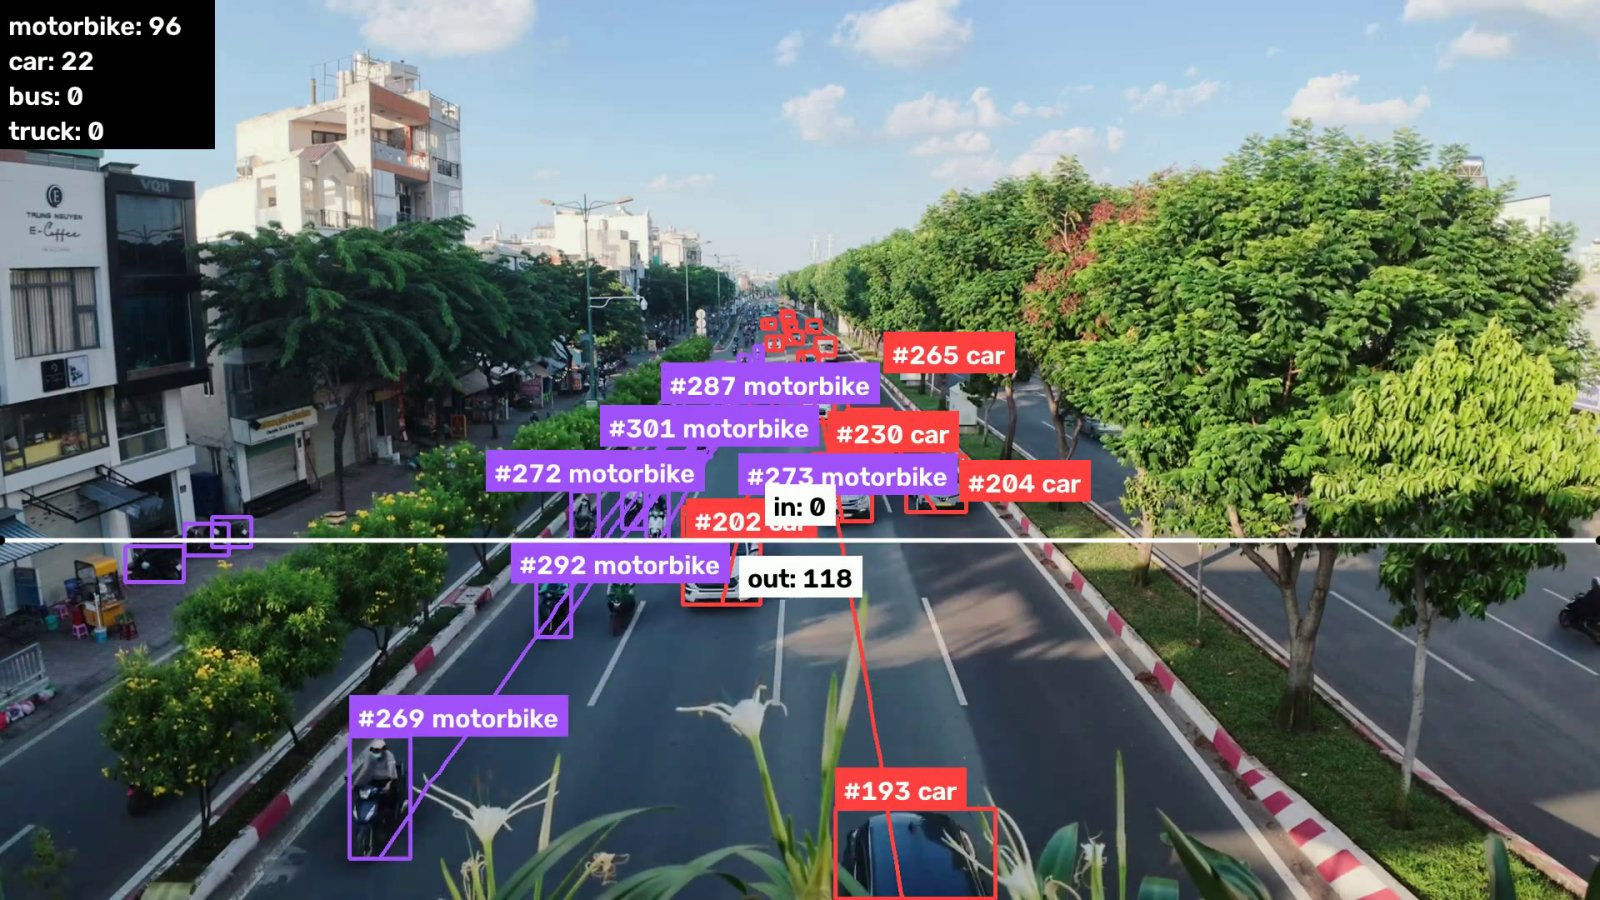
\includegraphics[width=\linewidth]{demo_pvd_goc_a.jpg}
  \caption{Một frame đầu ra của hệ thống trên clip đại lộ Phạm Văn Đồng (TP.HCM): box và nhãn ``\#ID lớp'' của từng
           xe, vết di chuyển, vạch đếm màu trắng và bảng đếm theo lớp ở góc trái (nguồn video: kênh YouTube Vietnam
           Naturally)}
  \label{fig:demo-pvd}
\end{figure}

\section{Ứng dụng của bài toán}

Hệ thống phát hiện, phân loại và theo dõi phương tiện là thành phần đầu vào của nhiều ứng dụng giao thông:
\begin{itemize}
  \item \textbf{Đếm lưu lượng.} Số xe qua một mặt cắt đường theo loại xe, theo hướng và theo thời gian. Đây là ứng dụng
        đề tài xây dựng và đánh giá sai số (mục~\ref{sec:dem-xe}).
  \item \textbf{Thống kê phục vụ quy hoạch và điều khiển tín hiệu.} Số liệu lưu lượng theo khung giờ giúp điều chỉnh
        chu kỳ đèn và đánh giá tải của nút giao.
  \item \textbf{Giám sát.} Quỹ đạo của từng xe là cơ sở để phát hiện các hành vi như đi ngược chiều hay dừng đỗ sai
        chỗ. Đề tài không làm các bài toán này nhưng đầu ra theo dõi có thể dùng lại cho chúng.
\end{itemize}

So với việc đếm thủ công hoặc dùng cảm biến đặt dưới mặt đường, cách làm dựa trên camera tận dụng được hạ tầng camera
có sẵn và cho biết thêm loại xe.

\section{Khó khăn và thách thức}
\label{sec:kho-khan}

Quá trình làm đề tài gặp sáu khó khăn chính; mỗi khó khăn dưới đây đi kèm số liệu đo được trong các chương sau.

\textbf{Thứ nhất, mật độ xe máy rất cao và che khuất lẫn nhau.} Tập test 30 frame cắt từ video ngã tư Hà Nội có 2.982
xe máy và 539 ô tô, tức khoảng 100 xe máy mỗi frame. Ở đèn đỏ, xe máy dừng sát nhau thành cụm, nhiều xe chỉ lộ ra một
phần. Đây là nơi mô hình bỏ sót nhiều nhất (Hình~\ref{fig:error-2}).

\textbf{Thứ hai, xe rất nhỏ ở xa.} Camera đặt cao nhìn dọc đại lộ thấy được cả đoạn đường dài, nên xe ở cuối đường chỉ
còn vài chục điểm ảnh. Trong tập test ban ngày \texttt{vn\_extra}, 52\% số xe có chiều cao dưới 32 điểm ảnh.

\textbf{Thứ ba, cảnh ban đêm.} Đèn pha và đèn hậu làm chói, thân xe tối màu lẫn vào nền, xe ở xa chỉ còn thấy đèn.
Mô hình dễ chỉ khoanh phần đèn sáng, hoặc nhầm xe máy chở hàng có đèn chói thành ô tô (mục~\ref{sec:phan-tich-loi}).

\textbf{Thứ tư, lệch miền dữ liệu.} Mô hình tốt trên tập test của bộ dữ liệu có sẵn chưa chắc tốt trên video mục tiêu.
Phiên bản v1 của đề tài đạt mAP50 0.861 trên tập test Roboflow nhưng trên frame Hà Nội AP50 của xe máy chỉ 0.045:
gần như không bắt được xe máy nhỏ của cảnh ngã tư.

\textbf{Thứ năm, thiếu dữ liệu đúng góc camera giao thông và định nghĩa lớp không thống nhất.} Các bộ dữ liệu có sẵn
phần lớn chụp ngang tầm mắt, từ drone hoặc từ một camera duy nhất. Mỗi bộ lại định nghĩa lớp theo cách riêng; ví dụ
xe van là \texttt{car} trong VisDrone nhưng là một lớp riêng trong KITTI và UA-DETRAC, còn xe Ford Transit 16 chỗ có
nơi xếp vào buýt, có nơi xếp vào ô tô.

\textbf{Thứ sáu, giới hạn tài nguyên.} Việc huấn luyện phụ thuộc hạn mức GPU của Kaggle; việc chạy demo diễn ra trên
laptop chỉ có CPU, nên mô hình phải đủ nhẹ. Mô hình chính xác nhất trong các thí nghiệm (RT-DETRv2-S) mất 1.53 giây
mỗi frame trên CPU, không dùng được cho video.

\section{Kết chương}

Chương này đã giới thiệu bài toán phát hiện, phân loại và theo dõi phương tiện từ video camera giao thông Việt Nam,
gồm ba bài toán con và ứng dụng đếm xe qua vạch. Các khó khăn chính là mật độ xe máy cao, xe nhỏ ở xa, cảnh đêm, lệch
miền dữ liệu, thiếu dữ liệu đúng góc camera và giới hạn phần cứng. Chương~\ref{chap:lythuyet} trình bày cơ sở lý
thuyết của các mô hình và chỉ số được dùng để giải quyết bài toán.
